\documentclass{article}
\usepackage[utf8]{inputenc} % Changed from utf8add to inputenc
\usepackage{amsmath}
\usepackage{geometry}
\usepackage{parskip}
\usepackage{cancel}
\usepackage{graphicx}
\usepackage{float}
\newcommand{\abs}[1]{\lvert#1\rvert} %this creates the vertical lines for "absolute value or the magnitude of a vector
\newcommand{\ezmatrix}[6]{
    \begin{vmatrix}
        \mathbf{i} & \mathbf{j} & \mathbf{k} \\
        #1 & #2 & #3 \\
        #4 & #5 & #6
    \end{vmatrix}
}
\newcommand{\vecgen}[3]{\langle #1, #2, #3 \rangle} %this creates the vector notation for the vector
\geometry{a4paper, margin=1in}

\title{Cross Product Notes}
\author{Christopher Greene}
\date{\today}

\begin{document}

\maketitle

% Cross product relationships
The unit vector cross products:
\begin{itemize}
    \item $\vec{i} \times \vec{j} = \vec{k}$
    \item $\vec{j} \times \vec{i} = -\vec{k}$
    \item $\vec{j} \times \vec{k} = \vec{i}$
    \item $\vec{k} \times \vec{j} = -\vec{i}$
    \item $\vec{k} \times \vec{i} = \vec{j}$
    \item $\vec{i} \times \vec{k} = -\vec{j}$
    \item $\vec{i} \times \vec{i} = \vec{0}$ (self cross product is zero)
\end{itemize}

\section*{General Cross Product Definition}
For vectors:
\begin{align*}
    \vec{u} &= u_1\vec{i} + u_2\vec{j} + u_3\vec{k} \\
    \vec{v} &= v_1\vec{i} + v_2\vec{j} + v_3\vec{k}
\end{align*}

The cross product expands as:
\begin{align*}
    \vec{u} \times \vec{v} &= (u_1\vec{i} + u_2\vec{j} + u_3\vec{k}) \times (v_1\vec{i} + v_2\vec{j} + v_3\vec{k}) \\
    &= u_1v_1(\cancel{\vec{i} \times \vec{i}} )0 + u_1v_2(\cancel{\vec{i} \times \vec{j}} )k + u_1v_3(\cancel{\vec{i} \times \vec{k}})-j \\
    &\quad + u_2v_1(\vec{j} \times \vec{i}) + u_2v_2(\vec{j} \times \vec{j}) + u_2v_3(\vec{j} \times \vec{k}) \\
    &\quad + u_3v_1(\vec{k} \times \vec{i}) + u_3v_2(\vec{k} \times \vec{j}) + u_3v_3(\vec{k} \times \vec{k})
\end{align*}

Using the self-cross product property $\vec{a} \times \vec{a} = \vec{0}$, this simplifies to:
\begin{align*}
    \vec{u} \times \vec{v} = &\ (u_2v_3 - u_3v_2)\vec{i} - (u_1v_3 - u_3v_1)\vec{j} + (u_1v_2 - u_2v_1)\vec{k}
\end{align*}

% 2D Matrices and Determinant
\begin{align*}
    \text{2D matrices:} \quad
    &\begin{vmatrix}
        a & b \\
        c & d 
    \end{vmatrix} \\
    \text{This yields:} \quad 
    &ad - bc \quad \text{(The result of this is called the determinant).}
\end{align*}

% 3D Matrices and Determinant
\begin{align*}
    \text{3D matrices:} \quad
    &\begin{vmatrix}
    \mathbf{i} & \mathbf{j} & \mathbf{k} \\
        a_1 & a_2 & a_3 \\
        b_1 & b_2 & b_3
    \end{vmatrix} \\
    \text{This yields:} \quad 
    &((a_2 b_3 - a_3 b_2)\vec{i} - (a_1 b_3 - a_3 b_1)\vec{j} + (a_1 b_2 - a_2 b_1)\vec{k}) \\
    \text{this can be broken down into:} \quad
    &\begin{vmatrix}
        a_2 & a_3 \\
        b_2 & b_3
    \end{vmatrix} \vec{i}
    - \begin{vmatrix}
        a_1 & a_3 \\
        b_1 & b_3
    \end{vmatrix} \vec{j}
    + \begin{vmatrix}
        a_1 & a_2 \\
        b_1 & b_2
    \end{vmatrix} \vec{k}
\end{align*}

\section*{Important takeaways:}

\begin{align*}
    \text{Let w equal the resultant vector from the cross product of u and v:} \\
    \vec{u} \times \vec{v} = \vec{w} \\
    \text{The resultant vector will be orthogonal to the plane which u and v are on.} \\
    \text{this vector w must be orthogonal to both u and v at any point} \\
    \text{this can be verified by using the dot poduct:} \\
    (\vec{u} \times \vec{v}) \cdot \vec{u} &= 0 \\
    \text{This must equal zero}
\end{align*}

\begin{figure}[H]
    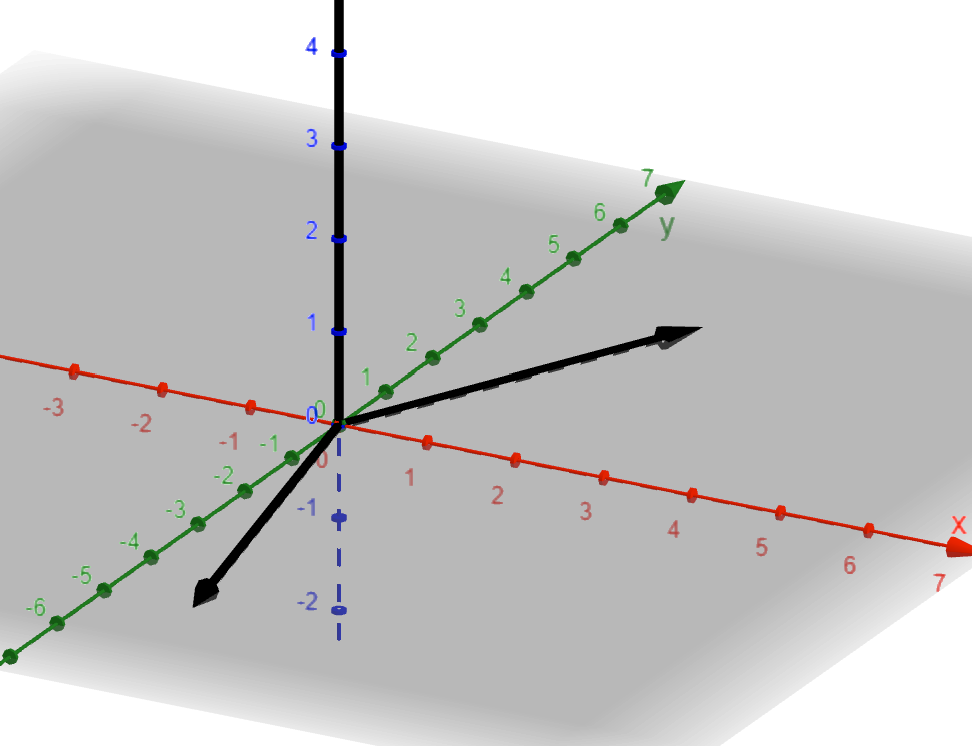
\includegraphics[scale=.5,trim=0 0 0 0]{crossProd.png} %trim[left,bottom,right,top]
    \caption{This shows the vector generated by the cross product}
\end{figure}

Important derivations: 
\begin{itemize}
    \item $\vec{u} \times \vec{v} = \abs{\vec{u}}\abs{\vec{v}}\cos$
    \item $\abs{\vec{u} \times \vec{v}} = \abs{\vec{u}} \abs{\vec{v}}\sin$
\end{itemize}

\section*{Examples:}

Example 1: Find the volume of the parallelepiped created by vectors u,v,w
\begin{align*}
    &\vec{u} = \vecgen{1}{-1}{1} \quad
    \vec{v} = \vecgen{1}{1}{2} \quad
    \vec{w} = \vecgen{-1}{-1}{1} \\
    &\text{recall that volume = (basearea) x (height)}\\
    &\text{base area = } \abs{\vec{u} \times \vec{v}} \\
    &\text{height = } \abs{\vec{w}} \\
    &\text{step 1. find} (\vec{u} \times \vec{v})\\
    \begin{vmatrix}
        \vec{i} & \vec{j} & \vec{k} \\
        1 & -1 & 1 \\
        1 & 1 & 2
    \end{vmatrix}
    &= \vec{i}(-1(2) - 1(1)) - \vec{j}(1(2) - 1(1)) + \vec{k}(1(1) - (-1)(1)) \\
    &= -3\vec{i} - \vec{j} + 2\vec{k} \\
    &\text{volume} = \vecgen{-3}{-1}{2} \times \text{height}\\
    &\text{step 2. find height}\\
    \text{height} = \vec{w}\\
    &\vecgen{-3}{-1}{2} \cdot \vecgen{-1}{-1}{1}\\
    &\text{volume} = ((-3)(-1)+(-1)(-1)+(2)(1)) \\
    &=(3+1+2)\\
    &\text{volume} = 6
\end{align*}

Example 2: Find the area of 2d triangle created by points P,Q,rangle
\begin{figure}[H]
    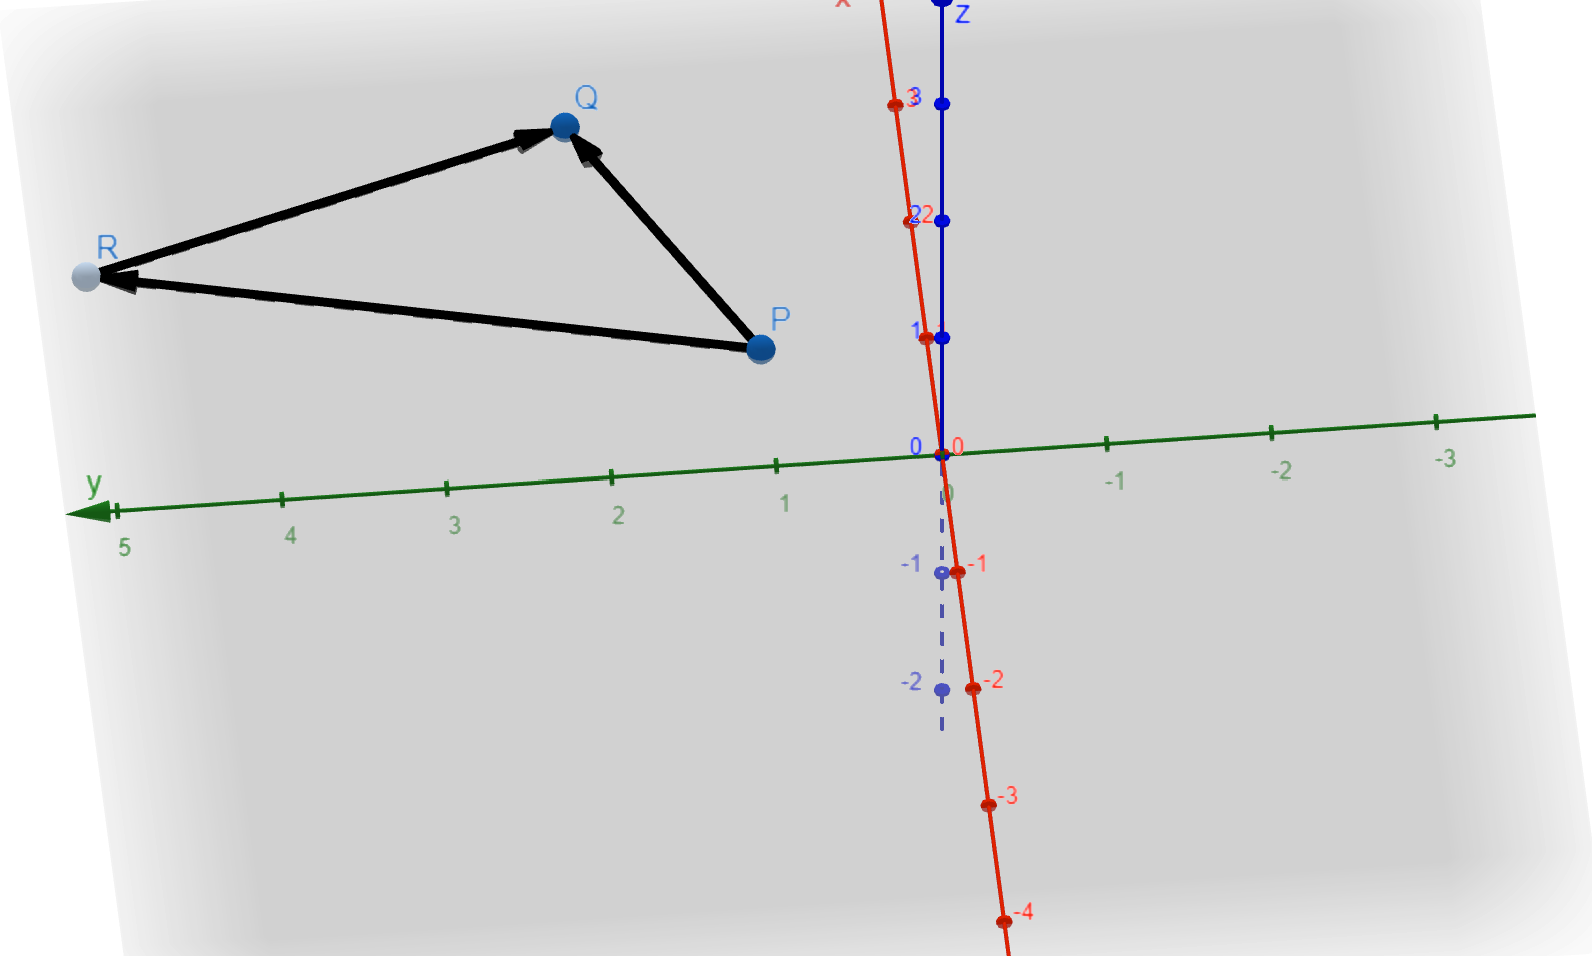
\includegraphics[scale=.5,trim=0 0 0 0]{triangle.png} %trim[left,bottom,right,top]
    \caption{This shows the triangle created by the points}
\end{figure}

\begin{align*}
    \begin{aligned}
    &\text{a parallelogram is created by 2 triangles.} \\
    &\text{Therefore  to get the area of the triangle we just need to find the area of the}\\
    &\text{parallelogram and divide by 2.}
    \end{aligned}
\end{align*}

\end{document}